%!TEX program = xelatex
%%%%%%%%%%%%%%%%%%%%%%%这是导言部分的开始%%%%%%%%

%========= 导言部分声明文档的类型=================
\documentclass{article}

%=========导言部分可可以加载宏包=================
\usepackage{amsmath}                % 数学公式排版宏包
\usepackage{amssymb}                % 数学符号命令宏包
\usepackage{amsthm}                 % 数学定理宏包
\usepackage[UTF8]{ctex}             % 中文输入宏包
\usepackage[a4paper]{geometry}      % 页面设置宏包
\usepackage{setspace}               % 行间距宏包
\usepackage{graphicx}               % 图片宏包
\usepackage{listings}               % 代码宏包
\usepackage{color}					% 颜色宏包
\usepackage{xcolor}                 % 颜色处理宏包
\usepackage{float}                  % 浮动对象式样宏包
\usepackage{fontspec}
\usepackage{enumerate}				% 列举编号包

%=========页面设置==============================
\geometry{left=1cm,right=1cm,top=1cm,bottom=2cm}
\onehalfspacing
\setlength\parindent{0em}

%=========代码格式设置============================
\definecolor{dkgreen}{rgb}{0,0.6,0}
\definecolor{gray}{rgb}{0.5,0.5,0.5}
\definecolor{mauve}{rgb}{0.58,0,0.82}
% \setmonofont{Consolas}
\lstset{
	numbers = left, 	
	numberstyle = \color{gray}, 
	keywordstyle = \color{blue},
	commentstyle = \color{dkgreen}, 
	stringstyle = \color{mauve},
	basicstyle = \ttfamily,
	breaklines = true,
	frame = shadowbox, % 阴影效果
	rulesepcolor = \color{ red!20!green!20!blue!20} ,
	escapeinside = ``, % 英文分号中可写入中文
	xleftmargin = 2em,xrightmargin=2em, aboveskip=1em,
	framexleftmargin = 2em
} 

%=========导言部分可以定义标题信息===============
\title{组会报告}
\author{徐益}
\date{\today}
%%%%%%%%%%%%%%%%%%%%%%%这是导言部分的结束%%%%%%%%%

%%%%%%%%%%%%%%%%%%%%%%%这是正文部分的开始%%%%%%%%%
\begin{document}

%=========生成标题================================
\maketitle

%=========开始正文的输入==========================

%===========第一节=================
\section{工作内容}
1. 提高信道估计和信号检测部分吞吐量;

2. 根据当前系统性能设计新的多线程系统;

3. 根据测试需求改写数据采集程序。

%===========第二节=================
\section{提高信道估计和信号检测部分吞吐量}
\subsection{优化要点}
\subsubsection{预先生成DCT矩阵}
\begin{figure}[H]
	\centering
	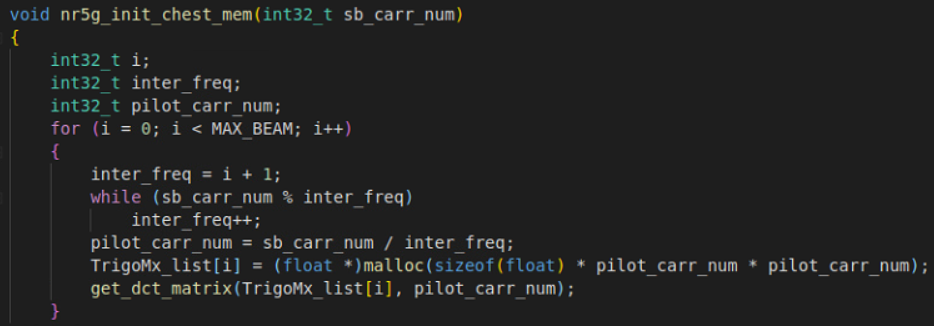
\includegraphics[width = .8\textwidth]{dct.png}
	\caption{信道估计初始化部分}
\end{figure}
\subsubsection{估计噪声时不做完整的DCT变换代码}
\begin{figure}[H]
	\centering
	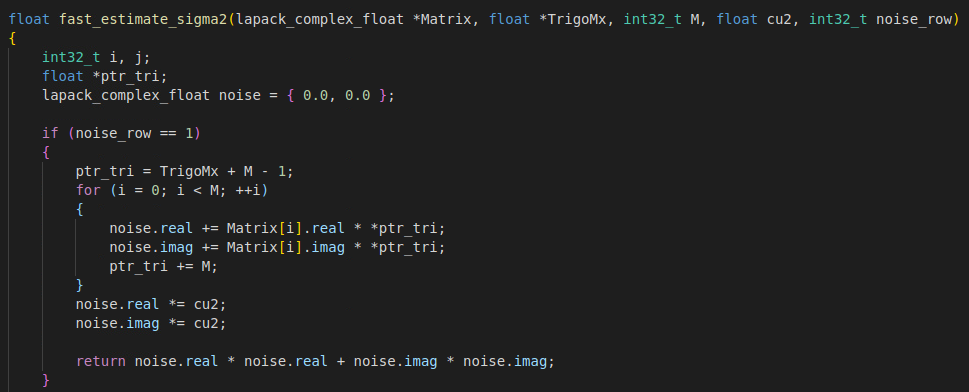
\includegraphics[width = .8\textwidth]{sigma.png}
	\caption{估计噪声部分代码}
\end{figure}
\subsubsection{指针移位寻址代替地址计算}
\begin{figure}[H]
	\centering
	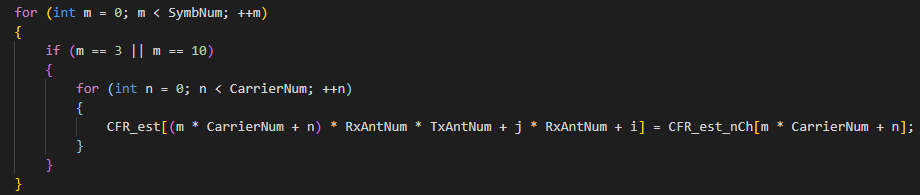
\includegraphics[width = .8\textwidth]{indx.png}
	\caption{原代码寻址部分}
\end{figure}
\begin{figure}[H]
	\centering
	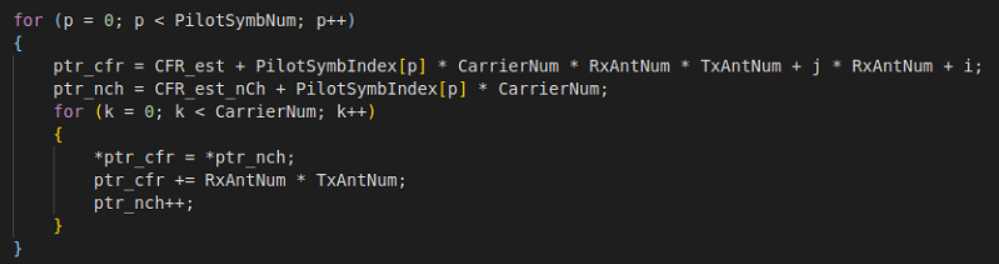
\includegraphics[width = .8\textwidth]{ptr.png}
	\caption{现代码寻址部分}
\end{figure}
\subsubsection{去除不必要的内部空间开辟}
\begin{figure}[H]
	\centering
	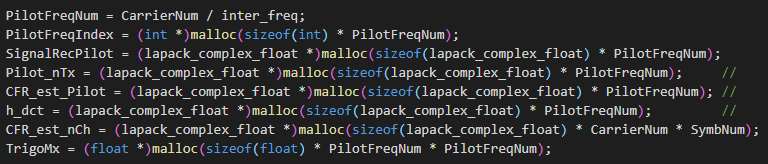
\includegraphics[width = .8\textwidth]{malloc.png}
	\caption{原代码中开辟空间部分}
\end{figure}

\subsection{优化成果}
\subsubsection{单流系统性能对比}
\begin{figure}[H]
	\centering
	\begin{minipage}[t]{0.48\textwidth}
		\centering
		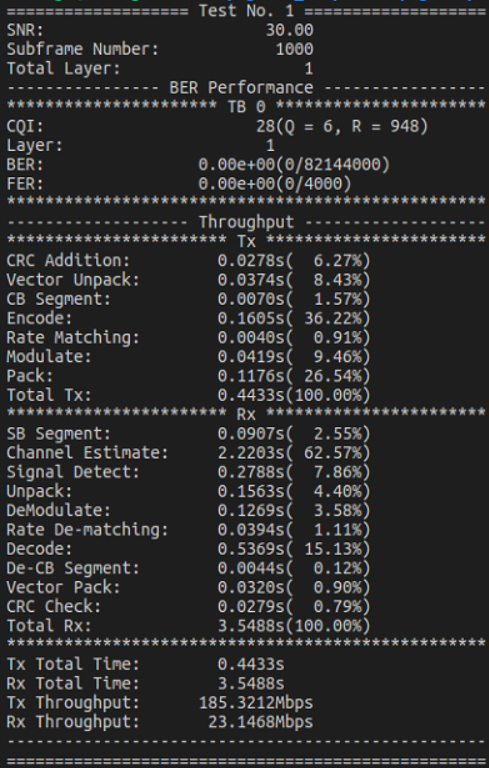
\includegraphics[width = \textwidth]{comp1.png}
		\caption{优化前}
	\end{minipage}
	\begin{minipage}[t]{0.48\textwidth}
		\centering
		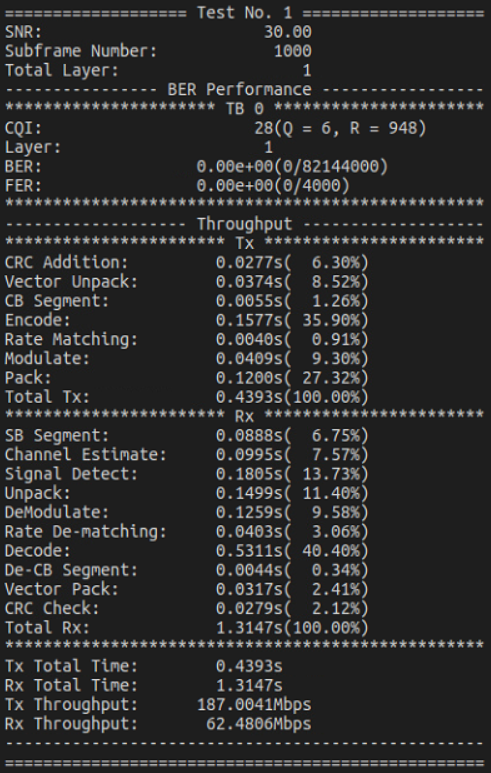
\includegraphics[width = \textwidth]{res1.png}
		\caption{优化后}
	\end{minipage}
\end{figure}
\subsubsection{八流系统性能对比}
\begin{figure}[H]
	\centering
	\begin{minipage}[t]{0.48\textwidth}
		\centering
		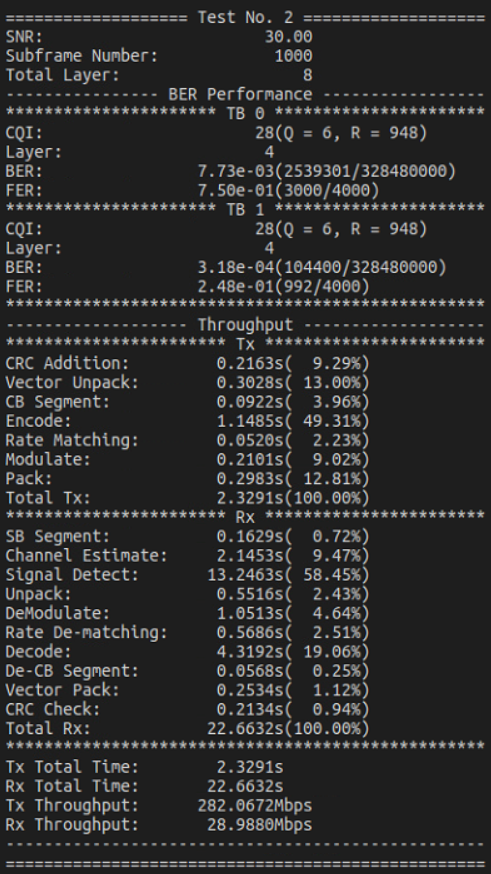
\includegraphics[width = \textwidth]{comp8.png}
		\caption{优化前}
	\end{minipage}
	\begin{minipage}[t]{0.48\textwidth}
		\centering
		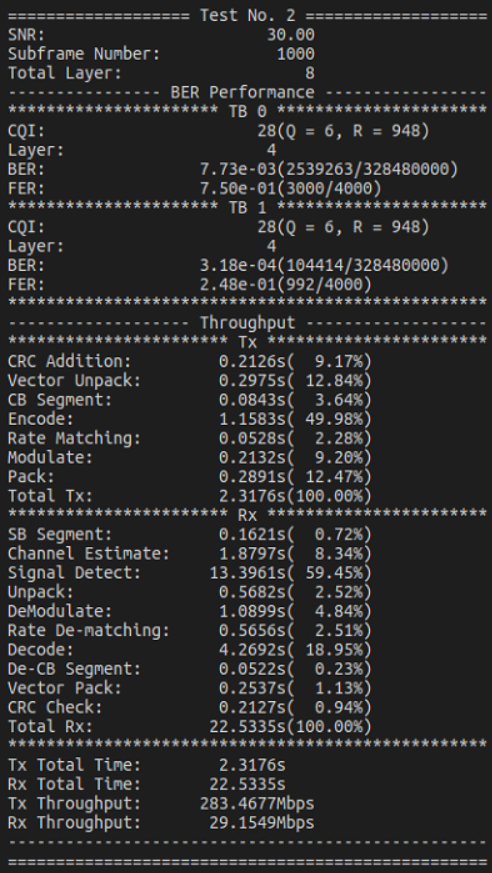
\includegraphics[width = \textwidth]{res8.png}
		\caption{优化后}
	\end{minipage}
\end{figure}

\subsection{仍存在的优化空间}
\begin{figure}[H]
	\centering
	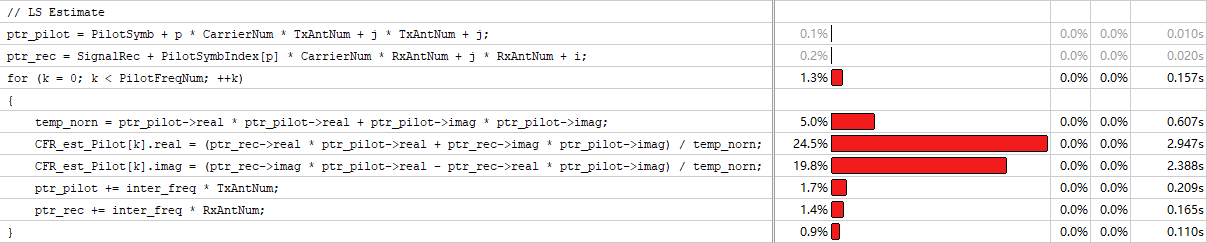
\includegraphics[width = .8\textwidth]{part1.png}
	\caption{信道估计复数除法部分}
\end{figure}
\begin{figure}[H]
	\centering
	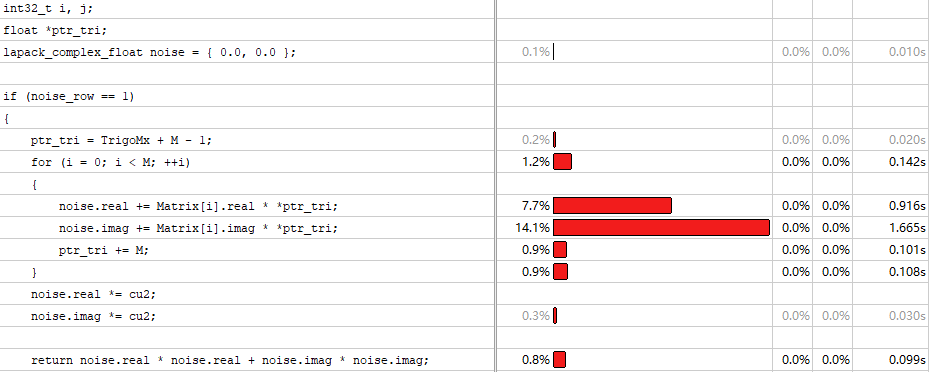
\includegraphics[width = .8\textwidth]{part2.png}
	\caption{估计噪声方差部分}
\end{figure}
%===========第三节=================
\section{新的多线程系统}
\begin{figure}[H]
	\centering
	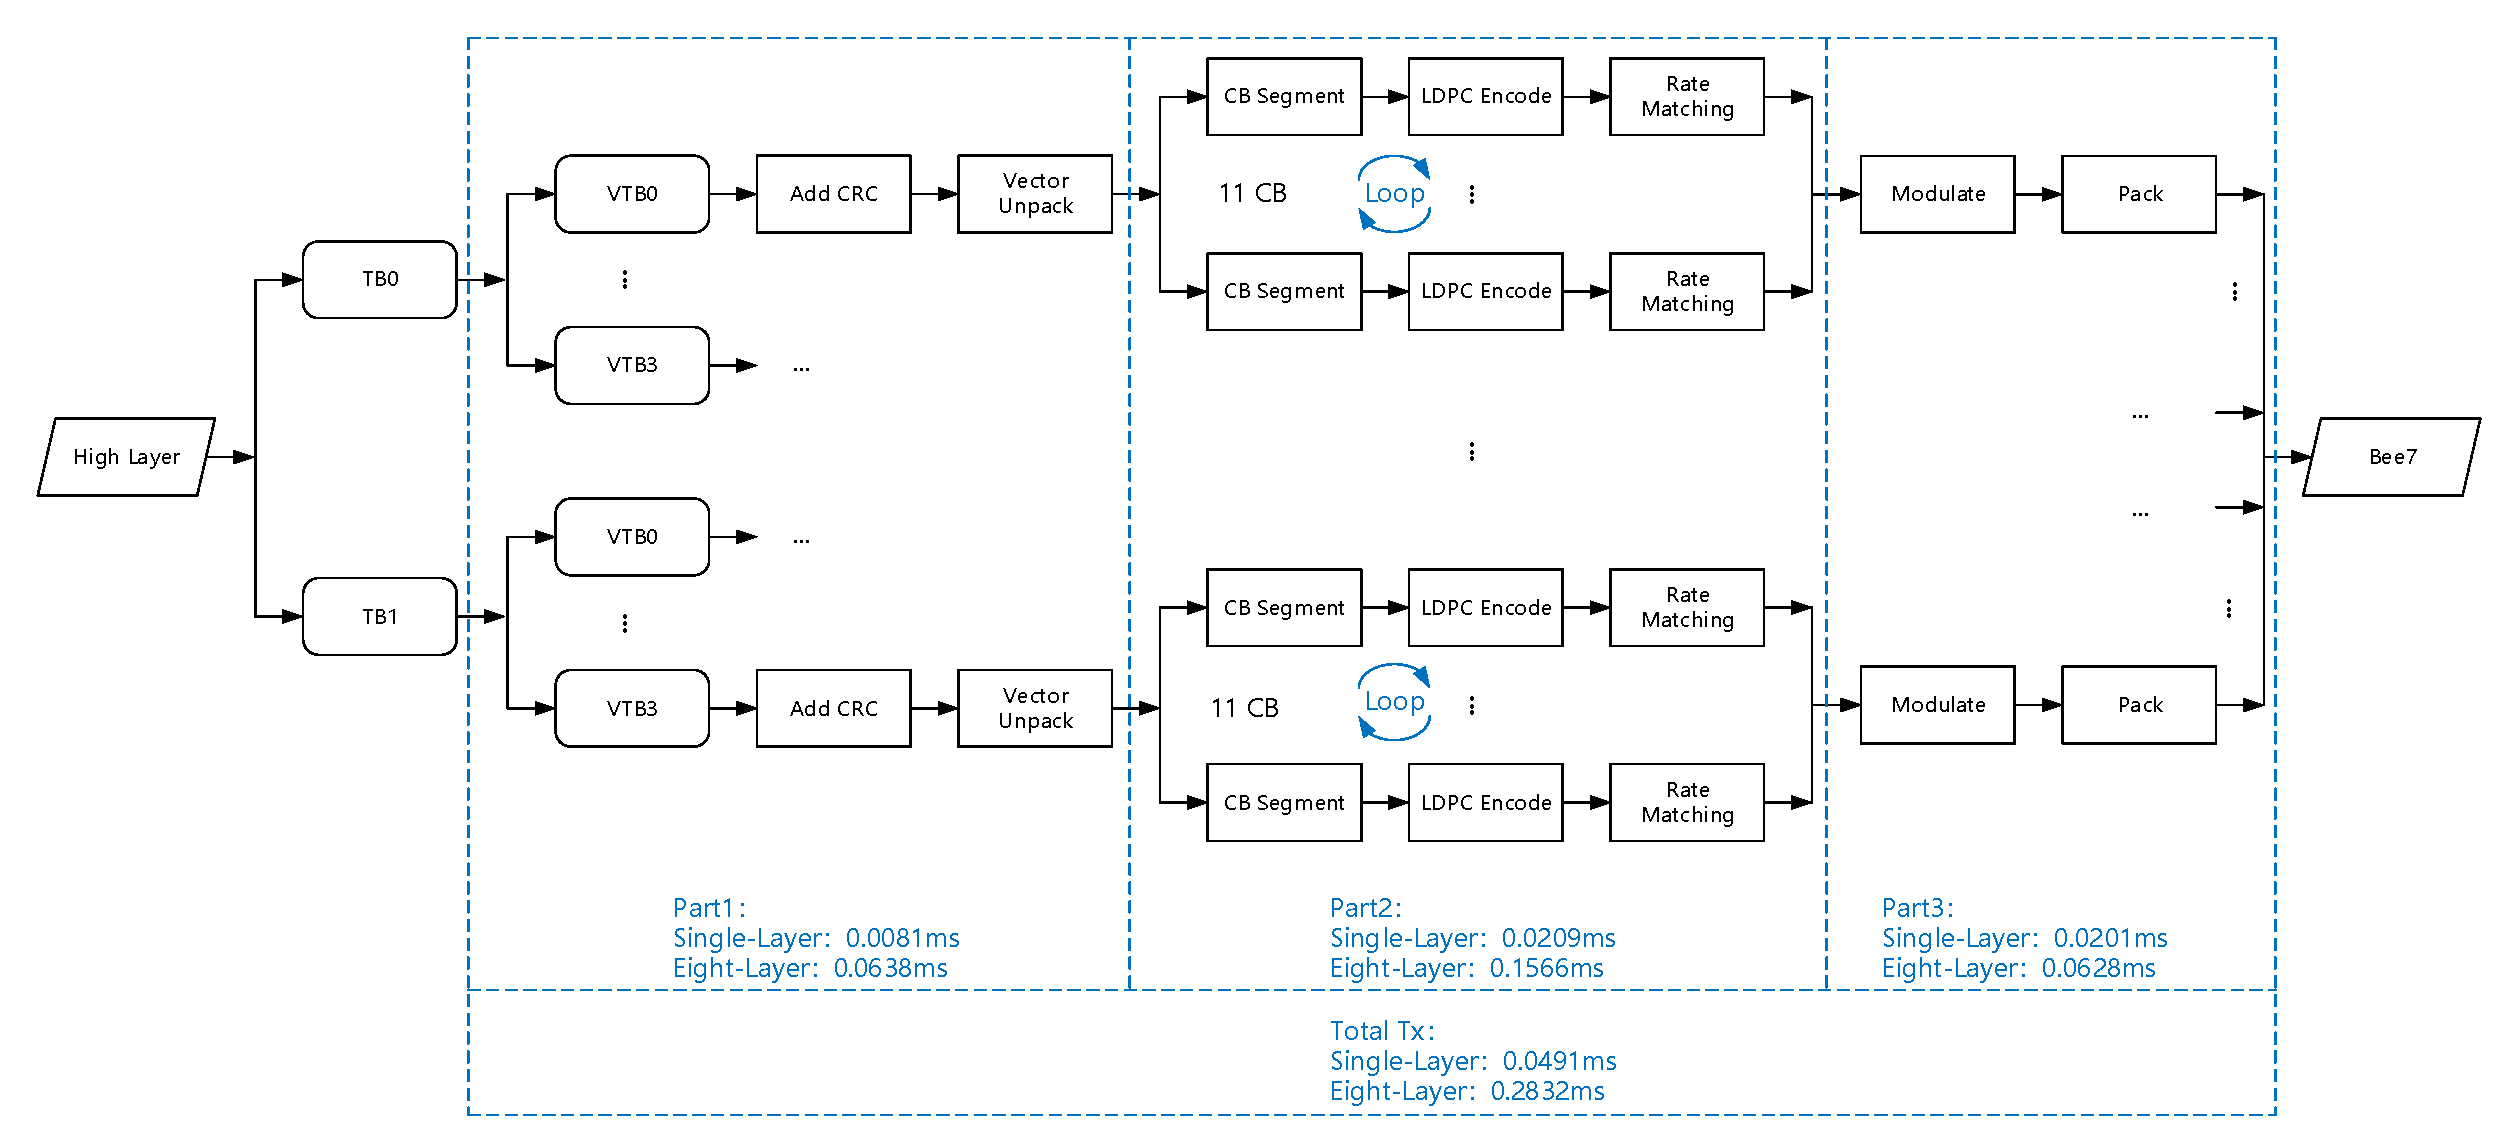
\includegraphics[width = \textwidth]{txstr.pdf}
	\caption{发送端}
\end{figure}
\begin{figure}[H]
	\centering
	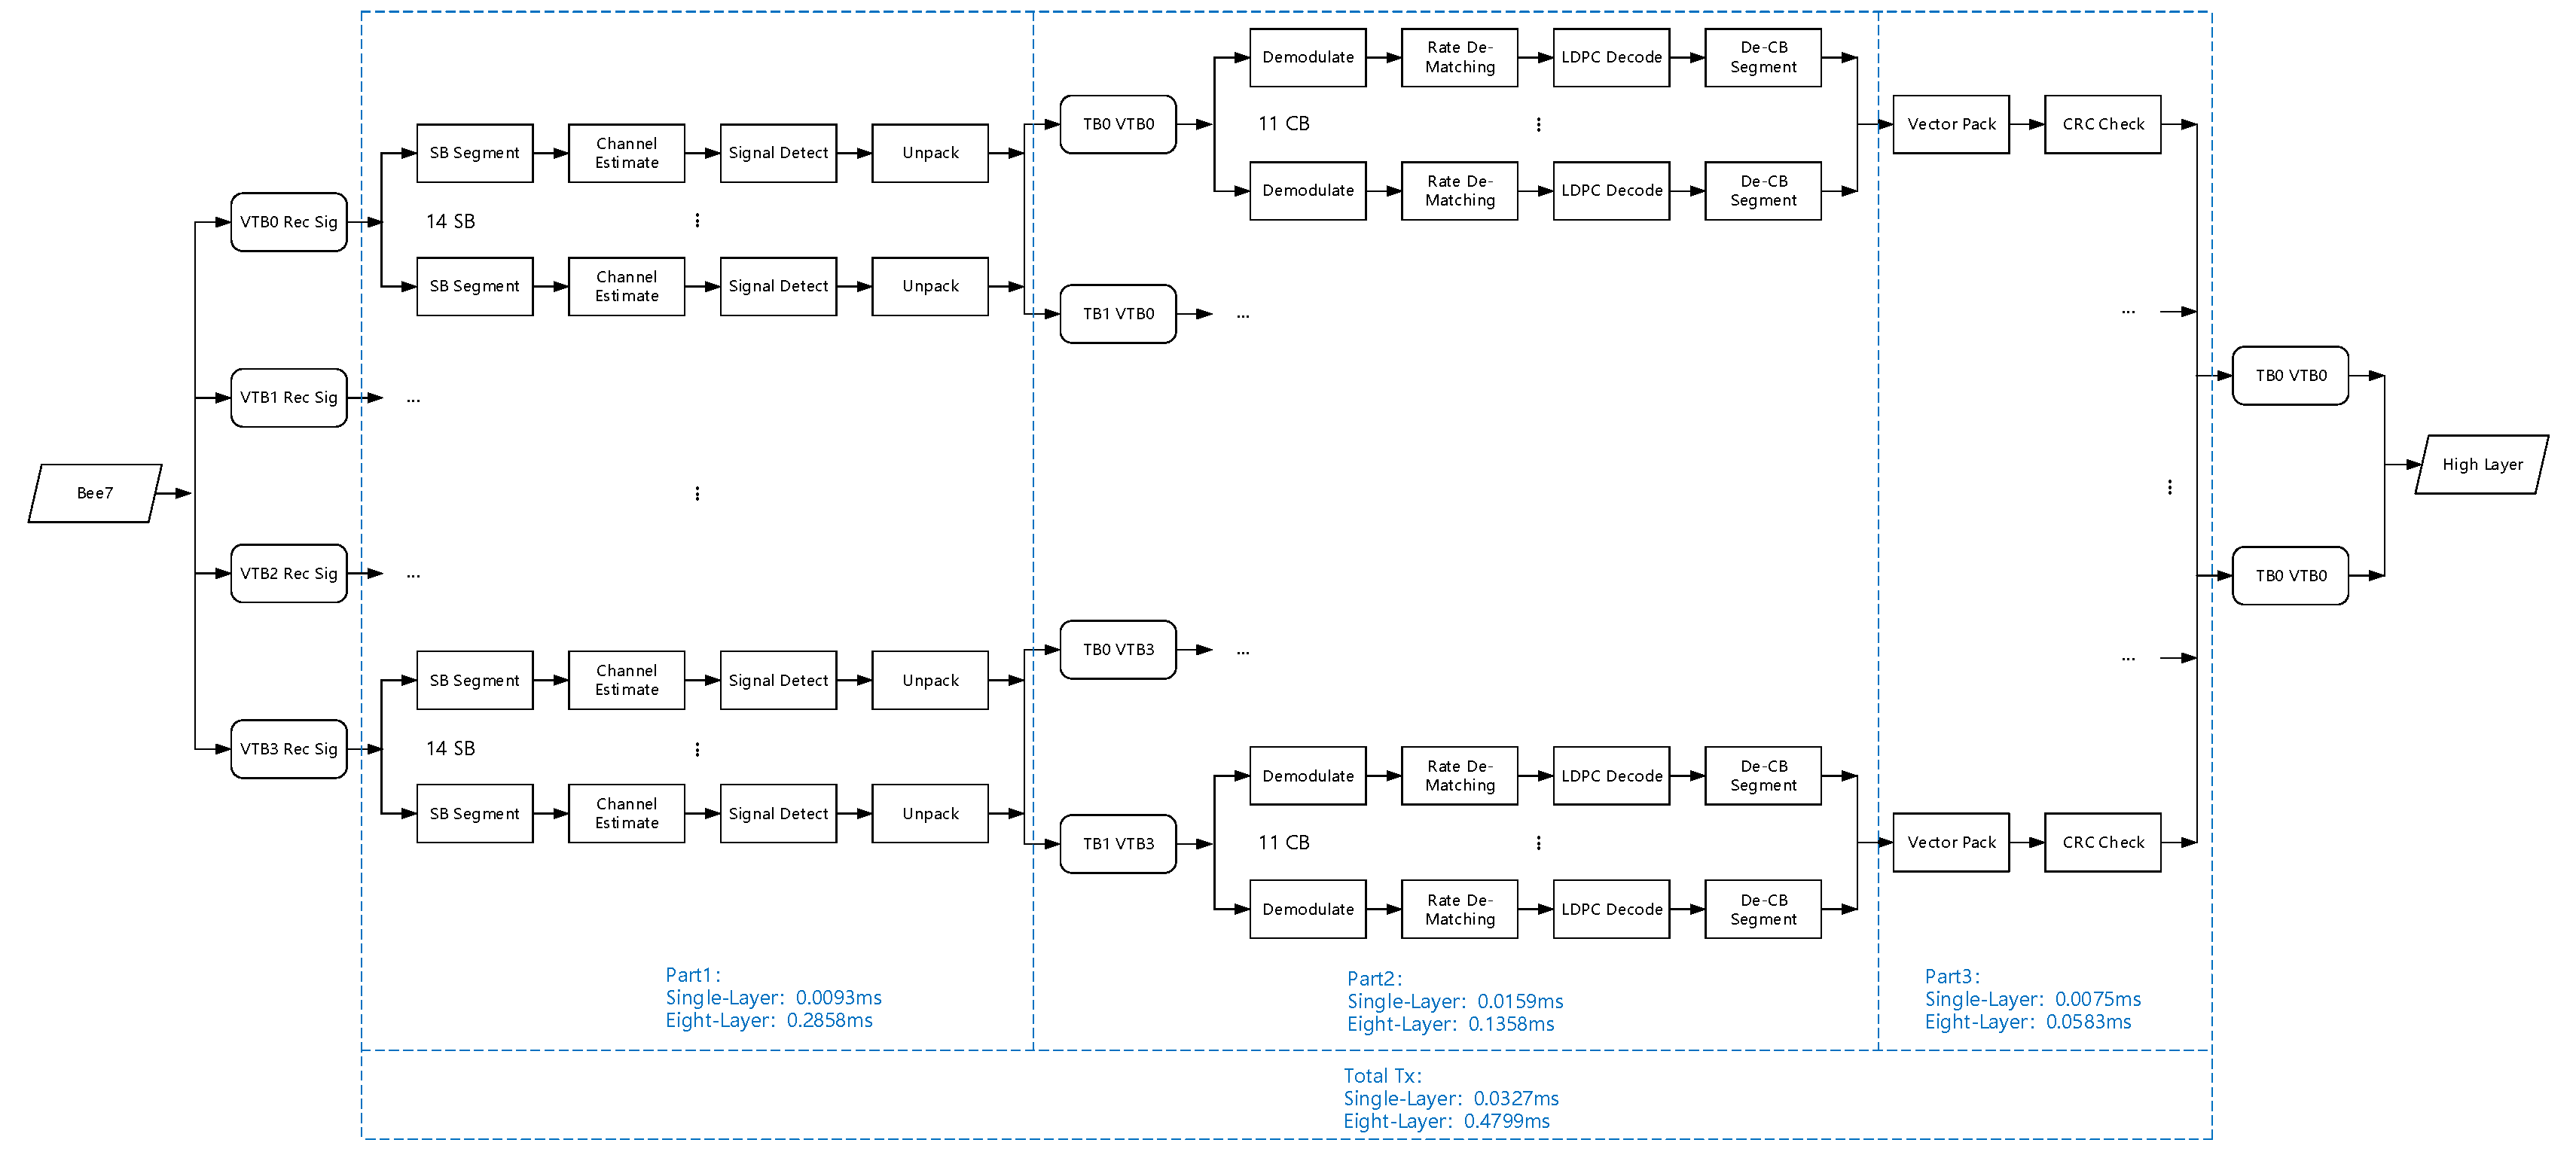
\includegraphics[width = \textwidth]{rxstr.pdf}
	\caption{接收端}
\end{figure}

%===========第四节=================
\section{修改数据采集程序}


%===========第五节=================
% \section{5GNR-LDPC报告}


%===========下周计划=================
\section{下阶段计划}
1. 根据当前架构修改与MAC层对接部分;

2. 根据当前架构修改多线程系统;

3. 参与MIMO信道测试。

\end{document}
%%%%%%%%%%%%%%%%%%%%%%%这是正文部分的结束%%%%%%%%%%%%